%%%%%%%%%%%%%%%%%%%%%%%%%%%%%%%%%%%%%%%%%%%%%%%%%%%%%%%%%%
% compiler: XeLaTeX
% TeX Live version: 2022
%%%%%%%%%%%%%%%%%%%%%%%%%%%%%%%%%%%%%%%%%%%%%%%%%%%%%%%%%%

\documentclass{SBCbookchapter}

%%%%%%%%%%%%%%%%%%%%%%%%%%%%%%%%%%%%%%%%%%%%%%%%%%%%%%%%%%
% packages
\usepackage[T1]{fontenc}
\usepackage[english]{babel}
\usepackage{graphicx}
\usepackage{amsmath,amsfonts,amssymb,mathrsfs}
\usepackage{txfonts}  % 可以不用
\usepackage{float}
\usepackage{multirow}
\usepackage{mathalfa}
\usepackage{enumitem}
\usepackage{bm}
\usepackage{relsize}
\usepackage[figurename=图, tablename=表]{caption}
\usepackage{csquotes}
\usepackage{chngcntr}
\counterwithin{figure}{section}
\counterwithin{table}{section}

\usepackage{arydshln}
\setlength{\dashlinegap}{2pt}
\setlength{\dashlinedash}{2pt}

% \usepackage[ruled,linesnumbered,algosection]{algorithm2e}
% \renewcommand*{\algorithmcfname}{算法}
% \renewcommand*{\algorithmautorefname}{算法}

% \makeatletter
% \renewcommand{\Indentp}[1]{%
%   \advance\leftskip by #1
%   \advance\skiptext by -#1
%   \advance\skiprule by #1}%
% \renewcommand{\Indp}{\algocf@adjustskipindent\Indentp{\algoskipindent}}
% \renewcommand{\Indpp}{\Indentp{0.5em}}%
% \renewcommand{\Indm}{\algocf@adjustskipindent\Indentp{-\algoskipindent}}
% \renewcommand{\Indmm}{\Indentp{-0.5em}}%
% \makeatother

\usepackage{algorithm,algorithmic}
\floatname{algorithm}{算法}

\usepackage{tikz}
\usetikzlibrary{trees,arrows.meta,decorations.pathmorphing,decorations.pathreplacing,shapes,shapes.geometric,backgrounds,positioning,calc,tikzmark,hobby,intersections}
% \usepackage{tkz-euclide}

\usepackage[slantfont,boldfont]{xeCJK}  % 这个只有用XeLaTeX编译才需要
%%%%%%%%%%%%%%%%%%%%%%%%%%%%%%%%%%%%%%%%%%%%%%%%%%%%%%%%%%


%%%%%%%%%%%%%%%%%%%%%%%%%%%%%%%%%%%%%%%%%%%%%%%%%%%%%%%%%%
% set chn font
% 这个在Windows下应该不需要
\setCJKmainfont{Noto Serif CJK SC}
\setCJKsansfont{Noto Sans CJK SC}
\setCJKmonofont{Noto Sans Mono CJK SC}
%%%%%%%%%%%%%%%%%%%%%%%%%%%%%%%%%%%%%%%%%%%%%%%%%%%%%%%%%%

% 参考文献工具,加载 biblatex 宏包,
% 其后端 backend 使用 biber,%标注(引用)样式 citestyle,
% 著录样式 bibstyle 都采用 gb7714-2015 样式,
% 两者相同时可以合并为一个选项 style
% https://ctan.org/pkg/biblatex-gb7714-2015?lang=en
% https://www.overleaf.com/learn/latex/Articles/Getting_started_with_BibLaTeX
\usepackage[backend=biber,style=gb7714-2015]{biblatex}
\addbibresource[location=local]{references.bib}


%%%%%%%%%%%%%%%%%%%%%%%%%%%%%%%%%%%%%%%%%%%%%%%%%%%%%%%%%%
% custom commands
\makeatletter
\newcommand{\mylabel}[2]{#2\def\@currentlabel{#2}\label{#1}}
\makeatother

\newcommand{\V}[1]{{\bm{#1}}}

\DeclareMathOperator*{\argmax}{arg\,max}
\DeclareMathOperator*{\argmin}{arg\,min}

% \algrenewcommand\algorithmicrequire{\textbf{Input:}}
% \algrenewcommand\algorithmicensure{\textbf{Output:}}

\newtheorem{thm}{定理}[section]
\newtheorem{prop}[thm]{命题}
\newtheorem{Def}[thm]{定义}
\newtheorem{lem}[thm]{引理}
\newtheorem{conj}[thm]{猜想}
\newtheorem{cor}[thm]{推论}
\newtheorem{remark}[thm]{注记}
\newtheorem{eg}[thm]{例}
\newtheorem{exam}[thm]{例}
\newtheorem{recall}[thm]{回忆}
\newtheorem{question}[thm]{问题}
\newtheorem{observation}[thm]{观察}

\newcommand{\R}{\mathcal{R}}

\numberwithin{equation}{section}

\renewcommand\arraystretch{1.3}

\allowdisplaybreaks

%%%%%%%%%%%%%%%%%%%%%%%%%%%%%%%%%%%%%%%%%%%%%%%%%%%%%%%%%%


\author{}
\title{特殊优化模型方法}

\setcounter{chapter}{7}

\setcounter{section}{2}

\begin{document}

\maketitle

%%%%%%%%%%%%%%%%%%%%%%%%%%%%%%%%%%%%%%%%%%%%%%%%%%%%%%%%%%
% main body
%%%%%%%%%%%%%%%%%%%%%%%%%%%%%%%%%%%%%%%%%%%%%%%%%%%%%%%%%%

\section{二次规划}
\label{sec:7.2}

% finished

具有二次目标函数和线性约束的约束优化问题被称为二次规划~(quadratic programming, QP) 问题. 这是一类非常常见的约束优化问题, 且它们也常常作为一般的约束优化问题的子问题出现. 二次规划问题的一般形式为
\begin{equation}
\label{eq:quadratic-programming-1}
\begin{array}{cl}
\min & q({x}) := \frac{1}{2} {x}^T G {x} + {d}^T {x}, \\
{\rm s.t.} & {a}_i^T {x} = b_i, ~~ i \in \mathcal{E} = \{1, \ldots, m_1\}, \\
& {a}_i^T {x} \leqslant b_i, ~~ i \in \mathcal{I} = \{m_1 + 1, \ldots, m\},
\end{array}
\end{equation}
其中~$G$ 是~$n$ 阶对称方阵, ${d}, {a}_i,$ 是~$n$ 维列向量, $b_i$ 是常数, $i \in \mathcal{E} \cup \mathcal{I},$ 约束条件有等式约束以及不等式约束. 以上形式的二次规划问题可以将约束条件以矩阵的形式表达为更加紧凑的形式:
\begin{equation}
\label{eq:quadratic-programming-2}
\begin{array}{cl}
\min & q({x}) := \frac{1}{2} {x}^T G {x} + {d}^T {x}, \\
{\rm s.t.} & A^T_{\mathcal{E}} {x} = {b}_{\mathcal{E}}, ~~ A^T_{\mathcal{I}} x \preccurlyeq {b}_{\mathcal{I}},
\end{array}
\end{equation}
其中~$A_{\mathcal{E}} = ({a}_1, \ldots, {a}_{m_1}), {b}_{\mathcal{E}} = (b_1, \ldots, b_{m_1})^T;$ $A_{\mathcal{I}} = ({a}_{m_1+1}, \ldots, {a}_m), {b}_{\mathcal{I}} = (b_{m_1+1}1, \ldots, b_m)^T.$ $A^T_{\mathcal{I}} {x} \preccurlyeq {b}_{\mathcal{I}}$ 表示
向量~$A^T_{\mathcal{I}} {b}_{\mathcal{I}}$ 的每个元素都小于等于向量~${b}_{\mathcal{I}}$ 相应位置元素. 问题~\eqref{eq:quadratic-programming-2} 的~KKT 条件为
\begin{equation}
\label{eq:quadratic-programming-kkt}
\begin{aligned}
& \nabla q({x}^*) + A {\lambda}^* = {0}, \\
& A^T_{\mathcal{E}} {x}^* - {b}_{\mathcal{E}} = {0}, \\
& {\lambda}^*_{\mathcal{I}} \succcurlyeq {0}, ~ A_{\mathcal{I}}^T {x}^* - {b}_{\mathcal{I}} \preccurlyeq {0}, ~ ({\lambda}^*_{\mathcal{I}})^T (A_{\mathcal{I}}^T {x}^* - {b}_{\mathcal{I}}) = {0},
\end{aligned}
\end{equation}
其中~$A = ({a}_1, \ldots, {a}_m);$ ${\lambda}^* = (\lambda_1^*, \ldots, \lambda_m^*)^T$ 为拉格朗日乘子, ${\lambda}^*_{\mathcal{I}} = (\lambda_{m_1+1}^*, \ldots, \lambda_m^*)^T;$ ${x}^*$ 为~KKT 点. 值得注意的是, 由于二次规划问题线性约束规范总成立, 二次规划问题的任一解都满足~KKT
条件~\eqref{eq:quadratic-programming-kkt}.

与线性规划问题类似, 一个二次规划问题总是能在有限步内求解, 或者证明其是不可行的或者无~(下) 界的. 当二次规划问题有解时, 若目标函数~$q({x}) = \frac{1}{2} {x}^T G {x} + {d}^T {x}$ 的~Hessian 阵~$G$ 是半正定的, 那么~$q({x})$ 是凸函数, 则该二次规划问题是凸规划问题, 其~KKT 点即为全局极小值点; 如果~$G$ 是正定的, 则解是唯一的~(唯一的全局极小值点). 当~$G$ 不定时, 目标函数~$q({x})$ 非凸, 可能有多个鞍点以及局部极小值点, 这些局部极小值点可能不是全局最优解. 此时, 求解全局最优解是一个~NP-难的问题~\cite{Murty_1987}.


\subsection{等式约束的二次规划问题}
\label{subsec:7.2.1}
% finished

首先考虑最简单的等式约束二次规划问题, 问题形式如下
\begin{equation}
\label{eq:quadratic-programming-eq-constrained}
\begin{array}{cl}
\min & q({x}) := \frac{1}{2} {x}^T G {x} + {d}^T {x}, \\
{\rm s.t.} & A^T {x} = {b},
\end{array}
\end{equation}
其中~$A = ({a}_1, \ldots, {a}_m)^T$ 是一个~$n \times m$ 的矩阵, ${a}_i \in \mathbb{R}^n,$ ${b} \in \mathbb{R}^m.$ 假设~$A$ 列满秩, 即~$A$ 的秩为~$m \leqslant n.$ 如若不然, 只需要去掉线性相关的约束即可.

求解等式约束的二次规划问题~\eqref{eq:quadratic-programming-eq-constrained} 的一个最直接的想法是通过等约束条件消去部分变量, 将问题化为无约束极小化问题进行求解. 将矩阵$A, G,$ 向量~${d}$,
以及变量~${x}$ 进行分块
\begin{equation}
\label{eq:quadratic-programming-eq-blocks}
A = \begin{bmatrix} A_1 \\ A_2 \end{bmatrix}, ~ G = \begin{bmatrix} G_{11} & G_{12} \\ G_{21} & G_{22} \end{bmatrix}, ~ {d} = \begin{bmatrix} {d}_1 \\ {d}_2 \end{bmatrix}, ~ {x} = \begin{bmatrix} {x}_1 \\ {x}_2 \end{bmatrix},
\end{equation}
其中~$A_1$ 是可逆的~$m$ 阶方阵, ${x}_1 \in \mathbb{R}^{m},$ ${x}_2 \in \mathbb{R}^{n-m},$
矩阵~$G$ 的分块以及向量~${d}$ 的分块与~${x}$ 的分块相容.
那么等式约束的二次规划问题~\eqref{eq:quadratic-programming-eq-constrained} 中的约束方程组~$A^T {x} = {b}$ 就可写作~$A_1^T {x}_1 + A_2^T {x}_2 = {b}.$ 由于~$A_1$ 可逆, 可以利用高斯消元法求解关于~${x}_1$ 的线性方程组~$A_1^T {x}_1 = {b} - A_2^T {x}_2$ 得唯一解
\begin{equation}
\label{eq:quadratic-programming-eq-constrained-subs}
{x}_1 = A_1^{-T} ({b} - A_2^T {x}_2).
\end{equation}
将上式代入目标函数~$q({x}),$ 可得关于~${x}_2$ 的二次函数
\begin{equation}
\begin{aligned}
\psi ({x}_2) := & \frac{1}{2} {x}_2^T \left( G_{22} - G_{21} A_1^{-T} A_2^T - A_2 A_1^{-1} G_{12} + A_2 A_1^{-1} G_{12} A_1^{-T} A_2^T \right) {x}_2 \\
& + {x}_2^T \left( G_{21} - A_2 A_1^{-1} G_{11} \right) A_1^{-T} {b} + \frac{1}{2} {b}^T A_1^{-1} G_{11} A_1^{-T} {b} \\
& + {x}_2^T \left( {d}_2 - A_2 A_1^{-1} {d}_1 \right) + {d}_1^T A_1^{-T} {b}.
\end{aligned}
\end{equation}
于是, 等式约束的二次规划问题~\eqref{eq:quadratic-programming-eq-constrained} 转化为了无约束极小化问题
\begin{equation*}
\min \quad \psi({x}_2)
\end{equation*}
如果~$\nabla^2 \psi$ 正定, 解~(一阶条件) 线性方程组~$\nabla \psi ({x}_2) = 0$
可得唯一解~${x}_2^*,$ 回代入~\eqref{eq:quadratic-programming-eq-constrained-subs} 可得~${x}_1^* = A_1^{-1} ( {b} - A_2 {x}_2^* ).$ 拉格朗日乘子~${\lambda}^*$ 由~KKT 条
件~\eqref{eq:quadratic-programming-kkt} 给出, 即由
\begin{equation}
\label{eq:quadratic-programming-eq-lambda}
\begin{bmatrix} A_1 \\ A_2 \end{bmatrix} {\lambda}^* = A {\lambda}^* = -\nabla q({x}^*) = - G {x}^* - {d} = - \begin{bmatrix} G_{11} & G_{12} \\ G_{21} & G_{22} \end{bmatrix} \begin{bmatrix} {x}_1^* \\ {x}_2^* \end{bmatrix} - \begin{bmatrix} {d}_1 \\ {d}_2 \end{bmatrix}
\end{equation}
确定. 解得拉格朗日乘子的显式表达
\begin{equation*}
{\lambda}^* = -A_1^{-1} \left( G_{11} {x}_1^* + G_{12} {x}_2^* + {d}_1 \right).
\end{equation*}

\begin{exam}\label{eg:7.2.1}
用直接消元法求解下列等式约束的二次规划问题
\begin{equation*}
\begin{array}{cl}
\min & q({x}) = x_1^2 + x_2^2 + 2x_3^2 + 5x_1x_2 - 3x_2 - 7x_3, \\
{\rm s.t.} & x_1 + x_2 + x_3 = 1, \\
& x_1 - 2x_2 - 3x_3 = -2,
\end{array}
\end{equation*}
那么相应的矩阵及其划分为
\begin{equation*}
A = \left[\begin{array}{@{}cc@{}} 1 & 1 \\ 1 & -2 \\ \hdashline 1 & -3 \end{array}\right], ~~ G = \left[\begin{array}{@{}cc:c@{}} 2 & 5 & 0 \\ 5 & 2 & 0 \\ \hdashline 0 & 0 & 4 \end{array}\right], ~~ {d} = \left[\begin{array}{@{}c@{}} 0 \\ -3 \\ \hdashline -7 \end{array}\right].
\end{equation*}
将约束条件写为
\begin{equation*}
\begin{aligned}
x_1 + x_2 & = 1 - x_3, \\
x_1 - 2x_2 & = -2 + 3x_3.
\end{aligned}
\end{equation*}
利用高斯消元法, 解得~$x_1 = \frac{1}{3} x_3, ~ x_2 = 1 - \frac{4}{3} x_3.$ 代入原目标函数得
\begin{equation*}
\psi(x_3) = \frac{5 x_{3}^{2}}{3} - 4 x_{3} - 2.
\end{equation*}
$\psi$ 的~{\rm Hessian} 阵~$\nabla^2 \psi = \psi'' = \frac{10}{3} > 0,$ 于是有唯一解. 由~$0 = \nabla \psi (x_3) = \frac{10 x_{3}}{3} - 4$ 解得~$x_3^* = \frac{6}{5}.$ 回代得~$x_1^* = \frac{2}{5},$ $x_2^* = -\frac{3}{5},$ 即~${x}^* = \left( \frac{2}{5}, -\frac{3}{5}, \frac{6}{5} \right)^T.$ 最后, 解方程组~\eqref{eq:quadratic-programming-eq-lambda}, 即
\begin{equation*}
\begin{bmatrix} 1 & 1 \\ 1 & -2 \\ 1 & -3 \end{bmatrix} ~ \begin{bmatrix} \lambda_1^* \\ \lambda_2^* \end{bmatrix} = - \begin{bmatrix} 2 & 5 & 0 \\ 5 & 2 & 0 \\ 0 & 0 & 4 \end{bmatrix} \begin{bmatrix} \frac{2}{5} \\ -\frac{3}{5} \\ \frac{6}{5} \end{bmatrix} - \begin{bmatrix} 0 \\ -3 \\ -7 \end{bmatrix},
\end{equation*}
算得拉格朗日乘子~$\lambda_1^* = \frac{11}{5}, \lambda_2^* = 0.$
\end{exam}

直接消元法是一种朴素初等的方法, 非常直观, 但不是求解等式约束二次规划
问题~\eqref{eq:quadratic-programming-eq-constrained} 的最优方法. 还可以采用广义消元法~(generalized elimination) 来求解. 这个方法的名字来源于矩阵的广义逆, 利用矩阵的广义逆来表
达问题~\eqref{eq:quadratic-programming-eq-constrained} 的等式约束~(线性方程组) $A^T {x} = {b}$ 的通解, 回代入目标函数~$q({x}),$ 得到一个无约束的极小化问题. 广义消元法的本质是对变量做了线性变换, 是直接消元法~\eqref{eq:quadratic-programming-eq-constrained-subs} 的推广.

对于非齐次线性方程组~$A^T {x} = {b},$ 它如果有解, 那么它的通解可以表示为
\begin{equation}
\label{eq:general-elim-1}
{x} = Y {b} + {s}
\end{equation}
其中~$Y \in \mathbb{R}^{n\times m}$ 是系数矩阵~$A^T$ 的某个广义逆, ${s}$ 是齐次线性方程组~$A^T {x} = 0$ 的解, 或者说属于~$A$ 的列零空间(null column space). ${s}$ 也被称作可行点~${x}$ 处的可行增量. $m\times n$ 的矩阵~$A^T$ 的广义逆, 指的是一个~$n\times m$ 的矩阵~$Y,$ 满足~$A^T Y A^T = A^T.$ 同时, 非齐次线性方程组~$A^T {x} = {b}$ 有解当且仅当~$A^T Y {b} = {b}.$ 假设取定了~$n \times m$ 的矩阵~$Y$ 以及~$n \times (n-m)$ 的矩阵~$Z,$ 满足
\begin{equation}
\label{eq:eq:general-elim-req}
\begin{bmatrix} Y & Z\end{bmatrix} \text{ 非奇异, 且~} A^T Y = I_m, ~ A^T Z = 0.
\end{equation}
也就是说~$Y$ 是~$A^T$ 的一个右广义逆~(比广义逆的定义~$A^T Y A^T = A^T$ 更进一步要求~$A^T Y = I_m$). 而矩阵~$Z$ 的列~${z}_1, \ldots, {z}_{n-m}$ 构成了~$A$ 的列零空间的一组基,
也被称作既约~(reduced) 坐标方向, 矩阵~$Z$ 也被称作零空间矩阵~(null-space matrix). 矩阵~$Z^T G Z$ 被称作二次规划问题~\eqref{eq:quadratic-programming-eq-constrained} 的既约~Hessian 阵. 那么,
可行增量~${s}$ 可以表示为~${z}_1, \ldots, {z}_{n-m}$ 的线性组合
\begin{equation}
\label{eq:general-elim-2}
{s} = Z {y} = \sum\limits_{i=1}^{n-m} y_i {z}_i,
\end{equation}
其中~$y_1, \ldots, y_{n-m}$ 是每个既约坐标方向的分量, 称~${y} = (y_1, \ldots, y_{n-m})^T$ 为既约变量. 将式~\eqref{eq:general-elim-2} 代入式~\eqref{eq:general-elim-1}, 于是每一个可行点~${x}$ 都可以表示为
\begin{equation}
\label{eq:general-elim-3}
{x} = Y {b} + Z {y}.
\end{equation}
这样, 就可以用既约变量~${y}$ 代换原变量~${x}$ 将等式约束消去, 将原问题转化为了无约束的既约二次函数的极小化问题
\begin{equation}
\label{eq:general-elim-4}
\min \quad \psi({y}) := \frac{1}{2} {y}^T Z^T G Z {y} + \left( {d} + G Y {b} \right)^T Z {y} + \frac{1}{2} \left( 2{d} + G Y {b} \right)^T Y {b}.
\end{equation}

下面解无约束的极小化问题~\eqref{eq:general-elim-4}. 考虑一阶条件
\begin{equation}
\label{eq:general-elim-5}
0 = \nabla \psi ({y}) = Z^T G Z {y} + Z^T \left( {d} + G Y {b} \right).
\end{equation}
如果既约~Hessian 阵~$Z^T G Z$ 是正定的, 那么有唯一解. 解关于~${y}$ 的线性方程组
\begin{equation}
\label{eq:general-elim-y}
Z^T G Z {y} = - Z^T \left( {d} + G Y {b} \right)
\end{equation}
得唯一解~${y}^*,$ 再代入变量替换式~\eqref{eq:quadratic-programming-eq-constrained-subs} 得到原问题的唯一解~${x}^* = Y {b} + Z {y}^*.$ 由~KKT 条件~\eqref{eq:quadratic-programming-kkt}, 拉格朗日乘子~${\lambda}^*$ 满足
\begin{equation}
\label{eq:general-elim-lagrange}
A {\lambda}^* = -\left( G {x}^* + {d} \right) =: - {g}^*,
\end{equation}
两边同时左乘~$Y^T,$ 有
\begin{equation}
\label{eq:general-elim-lambda}
{\lambda}^* = \left( A^T Y \right)^T {\lambda}^* = -Y^T {g}^*.
\end{equation}

到目前为止, 我们还没有介绍如何选取, 或者说构造矩阵~$Y$ 和~$Z.$ 这两个矩阵的构造方法有很多种, 通常首选的方法是正交分解法~(orthogonal factorization method): 对矩阵~$A$ 进行~QR 分解, 即
\begin{equation}
\label{eq:quadratic-programming-qr-decomp-1}
A = Q \begin{bmatrix} R \\ 0 \end{bmatrix} = \begin{bmatrix} Q_1 & Q_2 \end{bmatrix} \begin{bmatrix} R \\ 0 \end{bmatrix} = Q_1 R,
\end{equation}
其中~$Q$ 是~$n \times n$ 的正交阵, $R$ 是~$m \times m$ 的可逆上三角阵. $Q_1, Q_2$ 分别是~$n \times m$ 和~$n \times (n - m)$ 的矩阵. 然后选取
\begin{equation}
\label{eq:quadratic-programming-qr-decomp-2}
Y = Q_1 R^{-T}, ~~ Z = Q_2
\end{equation}
即可满足~\eqref{eq:eq:general-elim-req} 中关于矩阵~$Y,$ $Z$ 的要求. 通过解线性方程组
\begin{equation*}
R^T {v} = {b}
\end{equation*}
得到一个特解~${v},$ 进而可以得到~\eqref{eq:general-elim-3} 中的特解
\begin{equation*}
Y {b} = Y R^T {v} = Q_1 {v}.
\end{equation*}
接下来只要按照广义消元法的程序, 解关于既约变量~${y}$ 的方程组~\eqref{eq:general-elim-y} 得到唯一解~${y}^*,$ 回代得到原问题最优解~${x}^* = Y {b} + Z {y}^*,$
以及用式~\eqref{eq:general-elim-lambda} 计算得到相应的拉格朗日乘子.

矩阵~$Y,$ $Z$ 的通用计算格式如下: 任选一个~$n \times (n - m)$ 的矩阵~$V$ 使得~$\begin{bmatrix} A & V \end{bmatrix}$ 是非奇异的, 且逆可以分块表示为
\begin{equation}
\label{eq:quadratic-programming-qr-decomp-general}
\begin{bmatrix} A & V \end{bmatrix}^{-1} = \begin{bmatrix} Y^T \\ Z^T \end{bmatrix},
\end{equation}
其中~$Y$ 和~$Z$ 分别是~$n \times m$ 的矩阵和~$n \times (n - m)$ 的矩阵. 依照矩阵逆的定义, 有
\begin{equation*}
I_n = \begin{bmatrix} Y^T \\ Z^T \end{bmatrix} \begin{bmatrix} A & V \end{bmatrix} = \begin{bmatrix} Y^T A & Y^T V \\ Z^T A & Z^T V \end{bmatrix},
\end{equation*}
即有~$Y^T A = I_m, Z^T A = 0,$ 满足要求~\eqref{eq:eq:general-elim-req}, 适用于广义消元法. 这也可以解释之前介绍的直接消元法, 即如果取~$V = \begin{bmatrix} 0 \\ I_{n - m} \end{bmatrix},$
同时假设矩阵~$A$ 有形如~\eqref{eq:quadratic-programming-eq-blocks} 中的分块,
那么矩阵~$\begin{bmatrix} A & V \end{bmatrix}$ 的逆可以显式地表示为
\begin{equation*}
\begin{bmatrix} Y^T \\ Z^T \end{bmatrix} = \begin{bmatrix} A_1 & 0 \\ A_2 & I_{n - m} \end{bmatrix}^{-1} = \begin{bmatrix} A_1^{-1} & 0 \\ -A_2A_1^{-1} & I_{n - m} \end{bmatrix}.
\end{equation*}
这样就得到了之前的直接消元法. 此外, 如果取~$V = Q_2,$ 其中~$Q_2$ 由矩阵~$A$ 的~QR 分解
式~\eqref{eq:quadratic-programming-qr-decomp-1} 给出, 那么由
\begin{equation*}
\begin{bmatrix} Y^T \\ Z^T \end{bmatrix} = \begin{bmatrix} A & V \end{bmatrix}^{-1} = \begin{bmatrix} Q_1R & Q_2 \end{bmatrix}^{-1} = \begin{bmatrix} R^{-1} Q_1^T \\ Q_2^T \end{bmatrix}
\end{equation*}
可得正交分解法. 尽管关于矩阵~$Y$ 和~$Z$ 有各种各样的选取方式, 然而正交分解法通常是首选的. 原因之一是计算矩阵~$Z$ 时涉及正交矩阵的操作, 而正交矩阵具有良好的数值稳定性; 其次是选取~$Z = Q_2$ 可以给出条件数~$\kappa(Z^T G Z)$ 的最优上界, 即
\begin{equation*}
\kappa(Z^T G Z) \leqslant \kappa(G).
\end{equation*}

\begin{exam}\label{eg:7.2.2}
用广义消元法~$($正交分解法$)$ 来求解例~\eqref{eg:7.2.1} 中的二次规划问题. 首先得到约束条件系数矩阵的转置矩阵~$A$ 的~{\rm QR} 分解
\begin{equation*}
A = \begin{bmatrix} 1 & 1 \\ 1 & -2 \\ 1 & -3 \end{bmatrix} = \left[\begin{array}{@{}cc:c@{}} \frac{\sqrt{3}}{3} & \frac{7 \sqrt{78}}{78} & \frac{\sqrt{26}}{26} \\ \frac{\sqrt{3}}{3} & - \frac{\sqrt{78}}{39} & - \frac{2 \sqrt{26}}{13} \\ \frac{\sqrt{3}}{3} & - \frac{5 \sqrt{78}}{78} & \frac{3 \sqrt{26}}{26} \end{array}\right] ~ \left[\begin{array}{@{}cc@{}} \sqrt{3} & - \frac{4 \sqrt{3}}{3} \\ 0 & \frac{\sqrt{78}}{3} \\ \hdashline 0 & 0 \end{array}\right]
\end{equation*}
依照式~\eqref{eq:quadratic-programming-qr-decomp-2}, 令
\begin{equation*}
Y = \left[\begin{matrix} \frac{\sqrt{3}}{3} & \frac{7 \sqrt{78}}{78} \\ \frac{\sqrt{3}}{3} & - \frac{\sqrt{78}}{39} \\ \frac{\sqrt{3}}{3} & - \frac{5 \sqrt{78}}{78} \end{matrix}\right] ~ \left[\begin{matrix} \sqrt{3} & - \frac{4 \sqrt{3}}{3} \\ 0 & \frac{\sqrt{78}}{3} \end{matrix}\right]^{-T} = \frac{1}{26} \left[\begin{matrix} 18 & 7 \\ 6 & -2 \\ 2 & -5 \end{matrix}\right], ~~ Z = \frac{1}{\sqrt{26}} \left[\begin{matrix} 1 \\ -4 \\ 3 \end{matrix}\right].
\end{equation*}
此时, $Z^T G Z = \frac{15}{13} > 0,$ 有唯一解. 代入关于既约变量~$y$ 的线性
方程组~\eqref{eq:general-elim-y} 有
\begin{equation*}
\frac{15}{13} y = - Z^T \left( d + G Y b \right) = \frac{48 \sqrt{26}}{169},
\end{equation*}
解得~$y^* = \frac{16 \sqrt{26}}{65}.$ 回代得到原问题的最优解
\begin{equation*}
{x}^* = Y {b} + Z y^* = \left[\begin{matrix} \frac{2}{5} \\ - \frac{3}{5} \\ \frac{6}{5} \end{matrix}\right],
\end{equation*}
同时, 利用式~\eqref{eq:general-elim-lambda} 得到拉格朗日乘子
\begin{equation*}
{\lambda}^* = - Y^T \left( G {x}^* + {d} \right) = \left[\begin{matrix} \frac{11}{5} \\ 0 \end{matrix}\right].
\end{equation*}
这与例~\eqref{eg:7.2.1} 中用直接消元法得到的结果是一样的.
\end{exam}

还可以直接从等式约束的二次规划问题~\eqref{eq:quadratic-programming-eq-constrained} 的~KKT 条件入手,  来寻求该问题的解. 等式约束的二次规划问题的~KKT 条件可以从式~\eqref{eq:quadratic-programming-kkt} 简化为
\begin{equation}
\label{eq:quadratic-programming-kkt-2}
\begin{aligned}
& G {x}^* + {d} + A {\lambda}^* = {0}, \\
& A^T {x}^* - {b} = {0}.
\end{aligned}
\end{equation}
写为矩阵形式, 即为
\begin{equation}
\label{eq:quadratic-programming-kkt-2-mat}
\begin{bmatrix} G & A \\ A^T & 0 \end{bmatrix} \begin{bmatrix} {x}^* \\ {\lambda}^* \end{bmatrix} = \begin{bmatrix} -{d} \\ {b} \end{bmatrix}.
\end{equation}
上式中的系数矩阵~$K := \begin{bmatrix} G & A \\ A^T & 0 \end{bmatrix}$ 被称作拉格朗日矩阵,
也被称作~KKT 矩阵, 很容易看出~KKT 矩阵是对称不定的.
那么等式约束的二次规划问题~\eqref{eq:quadratic-programming-eq-constrained} 的求解就转化为了线性方程组~\eqref{eq:quadratic-programming-kkt-2-mat} 的求解.

如果~KKT 矩阵可逆, 将逆矩阵按相同的方式进行分块, 即
\begin{equation}
\label{eq:quadratic-programming-kkt-inverse}
\begin{bmatrix} G & A \\ A^T & 0 \end{bmatrix}^{-1} = \begin{bmatrix} C & E \\ E^T & F \end{bmatrix}
\end{equation}
那么~KKT 系统~\eqref{eq:quadratic-programming-kkt-2-mat} 的解就可写为
\begin{equation}
\label{eq:quadratic-programming-kkt-sol-1}
\begin{aligned}
{x}^* & = - C {d} + E {b}, \\
{\lambda}^* & = - E^T {d} + F {b}. \\
\end{aligned}
\end{equation}
当~$G$ 可逆时, 可以利用分块矩阵的消元法算得
\begin{equation}
\label{eq:quadratic-programming-kkt-inv-1}
\begin{aligned}
C & = G^{-1} - G^{-1} A \left( A^TG^{-1}A \right)^{-1} A^T G^{-1},\\
E & = G^{-1} A \left( A^TG^{-1}A \right)^{-1},\\
F & = - \left( A^TG^{-1}A \right)^{-1}.
\end{aligned}
\end{equation}
相关的方法被称作~Schur 补法~(Schur-complement method). 这个名字来源于, 执行分块消元操作的时候, 会得到矩阵~$G$ 的~Schur 补~$-A^TG^{-1}A.$ 要注意的是, Schur 补法要求~$G$ 可逆, 而这并不是~KKT 矩阵非奇异的必要条件; 同时基于数值稳定性等方面的考虑, 只有当~$G$ 正定以及~$A^TG^{-1}A$ 的计算开销足够小等一系列条件得到满足, Schur 补法才有应用的价值.

可以利用式~\eqref{eq:quadratic-programming-qr-decomp-general} 定义的矩阵~$Y,$ $Z$, 来求~KKT 矩阵的逆矩阵, 有
\begin{equation}
\label{eq:quadratic-programming-kkt-inv-2}
\begin{aligned}
C & = Z \left( Z^T G Z \right)^{-1} Z^T,\\
E & = Y - Z \left( Z^T G Z \right)^{-1} Z^T G Y,\\
F & = Y^T G Z \left( Z^T G Z \right)^{-1} Z^T G Y - Y^T G Y.\\
\end{aligned}
\end{equation}
这样, 可以利用矩阵~$Y,$ $Z$ 和~$Z^T G Z$ 的~Cholesky 分解~$L L^T$ 等计算方法来分解~KKT 矩阵, 相关的方法被称作零空间法~(null-space method). 这一名称来源于矩阵~$Z$ 的选取, 即~$Z$ 的列构成约束条件系数矩阵的转置矩阵~$A$ 的列零空间. 对应于不同的~$Y$ 和~$Z$ 的选取, 有不同的零空间法, 如上面介绍的广义消元法.


\subsection{求解二次规划问题的积极集法}
\label{subsec:7.2.2}
% finished

对于一般的带不等式约束的二次规划问题~\eqref{eq:quadratic-programming-1}, 有一系列的实用算法来求解这些问题. 经典的积极集法~(active-set methods) 自从~20 世纪~70 年代起被广泛应用于求解二次规划问题. 积极集法适用于求解中小规模~(成百上千个变量) 的凸和非凸的二次规划问题. 梯度投影法~(gradient-projection methods) 是属于积极集法的一种特殊的算法, 是经典积极集法的推广, 能够非常高效地求解简单约束的二次规划问题, 例如对每个变量的约束都是区间约束的二次规划问题~($a_i \leqslant x_i \leqslant b_i,$ 称这样的问题为~BoxQP). 还有一类方法是内点法~(interior-point methods), 这类方法被广泛应用于求解二次规划问题的时间比经典积极集法稍晚, 大概始于~20 世纪~90 年代. 内点法适用于求解大规模的凸二次规划问题.

本节主要介绍如何利用积极集法将等式约束问题的求解方法推广以求解带不等式约束的二次规划问题. 为描述简单, 假设原问题是凸二次规划问题. 回顾一下, 对于二次规划问题~\eqref{eq:quadratic-programming-1}, 积极集~$\mathcal{A}(x)$ 的定义为
\begin{equation}
\label{eq:qp-active-set}
\mathcal{A} = \mathcal{A}({x}) = \left\{ i : ~ {a}_i^T {x} = b_i, ~ i \in \mathcal{E} \cup \mathcal{I} \right\},
\end{equation}
即在点~${x}$ 处, 等式成立的约束条件的指标~(index) 组成的集合.
将一般的二次规划的~KKT 条件~\eqref{eq:quadratic-programming-kkt} 根据积极集~$\mathcal{A}({x}^*)$ 改写一下, 即有
\begin{equation}
\label{eq:qp-active-set-kkt}
\begin{aligned}
& G {x}^* + d + \sum\limits_{i \in \mathcal{A}({x}^*)} \lambda_i^* {a}_i = {0}, \\
& {a}_i^T {x}^* = b_i, ~~ \forall i \in \mathcal{A}({x}^*), \\
& {a}_i^T {x}^* \leqslant b_i, ~~ \forall i \in \mathcal{I} \setminus \mathcal{A}({x}^*), \\
& \lambda_i^* \geqslant 0, ~~ \forall i \in \mathcal{I} \cap \mathcal{A}({x}^*).
\end{aligned}
\end{equation}
不难发现, ${x}^*$ 也是下面等式问题的~KKT 点
\begin{equation}
\label{eq:qp-active-set-1}
\begin{array}{cl}
\min & \frac{1}{2} {x}^T G {x} + {d}^T {x}, \\
{\rm s.t.} & {a}_i^T {x} = b_i, ~ i \in \mathcal{A}({x}^*).
\end{array}
\end{equation}
这说明, 如果事先知道最优点处的积极集~$\mathcal{A}({x}^*),$ 那么求解含不等式约束的二次规划问题几乎~(注意~KKT 条件~\eqref{eq:qp-active-set-kkt} 中的最后两个条件) 等价于求解一个等式约束的二次规划问题. 但通常这是不可能的, 因此不能通过求解等式问题~\eqref{eq:qp-active-set-1} 来求解原二次规
划问题~\eqref{eq:quadratic-programming-1}.

在积极集法中, 依据以上的观察, 我们将积极集~$\mathcal{A}$ 确定的约束看作等式约束, 而暂时忽略其余约束条件, 并通过某种迭代的方式不断修正调整这个集合, 直到识别出原问题~\eqref{eq:quadratic-programming-1} 的解处的正确的积极约束. 更具体来说, 在第~$k$ 次迭代, 从可行点~${x}^{(k)}$ 出发,
积极集为~$\mathcal{A} = \mathcal{A}({x}^{(k)}).$ 在这一步迭代中,
求解等式问题~\eqref{eq:qp-active-set-1}. 更方便的做法是将原点平移到~${x}^{(k)},$ 令~${s} = {x} - {x}^{(k)},$ 求解问题
\begin{equation}
\label{eq:qp-active-set-2}
\begin{array}{cl}
\min & \frac{1}{2} {s}^T G {s} + \left( {g}^{(k)} \right)^T {s}, \\
{\rm s.t.} & {a}_i^T {s} = 0, ~ i \in \mathcal{A},
\end{array}
\end{equation}
其中
\begin{equation*}
{g}^{(k)} = \nabla q({x}^{(k)}) = G {x}^{(k)} + {d}
\end{equation*}
是原二次规划问题~\eqref{eq:quadratic-programming-1} 的目标函数~$q({x})$ 在点~${x}^{(k)}$ 处的梯度向量.  这个问题是一个等式约束的二次规划问题, 可以用上一小节~\S\ref{subsec:7.2.1} 中介绍的等式约束二次规划问题的求解方法进行求解. 记问题~\eqref{eq:qp-active-set-2} 的解为~${s}^{(k)},$ 需要对各种可能的情况进行分类讨论.

第一种情况是~${s}^{(k)} = {0},$ 即~${x}^{(k)}$ 是当前等式约束问题~\eqref{eq:qp-active-set-1} 的解, 那么可以根据式~\eqref{eq:general-elim-lagrange} 计算积极约束的拉格朗日乘子, 记为~${\lambda}^{(k)},$  即有
\begin{equation}
\label{eq:qp-active-set-lambda}
{g}^{(k)} + \sum\limits_{i \in \mathcal{A}} \lambda_i^{(k)} a_i = 0.
\end{equation}
此时, 除对偶可行性条件~$\lambda_i \geqslant 0, ~ i \in \mathcal{I}$ 以外, 其余~KKT
条件~\eqref{eq:qp-active-set-kkt} 均满足. 当与原问题不等式约束对应的拉格朗日乘子均非负, 即
\begin{equation*}
\lambda_i^{(k)} \geqslant 0, ~ \forall i \in \mathcal{I} \cap \mathcal{A},
\end{equation*}
则~$x^{(k)}$ 是原问题的~KKT 点, 迭代结束, 求解完毕. 如若不然, 即有一个或多个拉格朗日乘子取负值,
这时候一个有效的策略是从积极集中去掉某一个负的拉格朗日乘子对应的约束条件, 并求解由此得到的新的等式约束问题, 相应的解可以使目标函数值下降. 一般我们取
\begin{equation}
\label{eq:qp-active-set-inactive-index}
q = \argmin_{i \in \mathcal{I} \cap \mathcal{A}} \lambda_i^{(k)},
\end{equation}
有~$\lambda_q^{(k)} < 0.$ 令~$\mathcal{A} = \mathcal{A} \setminus \{ q \},$
代入问题~\eqref{eq:qp-active-set-2}, 并求解此新的等式约束问题. 可以证明, 这个新的等式约束问题的解,
暂记为~$s,$ 的确是我们去掉的第~$q$ 个约束条件的可行方向, 即有~$a_p^T s \geqslant 0$ (去掉其它任何一个负的拉格朗日乘子对应的约束条件得到的等式约束问题解得的解, 都是相应约束条件的可行方向). 更进一步地, 若~$s$ 还满足一些好的条件, 例如二阶最优性充分条件, 那么~$s$ 会是目标函数的~(严格) 下降方向.

第二种情况是~${s}^{(k)} \neq {0},$ 即~${x}^{(k)}$ 不是当前等式约束问题~\eqref{eq:qp-active-set-1} 的解, 那么我们需要进一步检验试探点
\begin{equation}
\label{eq:qp-active-set-test-point}
\bar{{x}}^{(k)} = {x}^{(k)} + {s}^{(k)}
\end{equation}
是否满足其他不在积极集~$\mathcal{A}$ 中的不等式约束条件. 如果都满足的话, 令
\begin{equation}
\label{eq:qp-active-set-next-step-1}
{x}^{(k+1)} = \bar{{x}}^{(k)} = {x}^{(k)} + {s}^{(k)},
\end{equation}
积极集保持不变, 进入下一步迭代搜索. 如若不然, 即存在指标~$i \not\in \mathcal{A},$ 使得
\begin{equation*}
{a}_i^T {x}^{(k)} - {b} + {s}^{(k)} > 0,
\end{equation*}
此时试探点~$\bar{{x}}^{(k)}$ 不是原问题的可行点, 需要将其投影到原问题的可行域.
一个自然的想法是, 沿着方向~${p}^{(k)} = {s}^{(k)}$ 进行线搜索, 选一个小于~$1$ 但尽可能大的步长
\begin{equation}
\label{eq:qp-active-set-step-len-1}
\begin{aligned}
\bar{\alpha}_k & = \max \left\{ \alpha : ~ \alpha > 0, ~ {a}_i^T {x}^{(k)} - b_i + \alpha {a}_i^T {p}^{(k)} \leqslant 0, ~ {a}_i^T {p}^{(k)} > 0, ~ \forall i \not\in \mathcal{A} \right\}, \\
& = \min_{\substack{i: i \not\in \mathcal{A} \\ {a}_i^T {p}^{(k)} > 0}} \frac{b_i - {a}_i^T {x}^{(k)}}{{a}_i^T {p}^{(k)}}.
\end{aligned}
\end{equation}
注意~$\bar{\alpha}_k$ 是严格小于~$1$ 的, 因为此时的试探点~${x}^{(k)} + {s}^{(k)}$ 不可行. 取指标~$j$ 使得第~$j$ 个约束取得上式中~$\frac{b_i - {a}_i^T {x}^{(k)}}{{a}_i^T {p}^{(k)}}$ 的最大值, 即
\begin{equation}
\label{eq:qp-active-set-step-len-2}
j = \argmin_{\substack{i: i \not\in \mathcal{A} \\ {a}_i^T {p}^{(k)} > 0}} \frac{b_i - {a}_i^T {x}^{(k)}}{{a}_i^T {p}^{(k)}}, ~~ \bar{\alpha}_k = \frac{b_j - {a}_j^T {x}^{(k)}}{{a}_j^T {p}^{(k)}},
\end{equation}
并称指标~$j$ 对应的约束为阻滞~(blocking) 约束. 取下一步迭代点为
\begin{equation}
\label{eq:qp-active-set-next-step-2}
{x}^{(k+1)} = {x}^{(k)} + \bar{\alpha}_k {s}^{(k)}, ~~ \mathcal{A} \gets \mathcal{A} \cup \{ j \}.
\end{equation}
这里把指标~$j$ 添加到了积极集, 是因为对于~${x}^{(k+1)},$ 指标~$j$ 对应的约束条件等式成立, 非积极约束~$j$ 变成积极的. 迭代格式~\eqref{eq:qp-active-set-next-step-1}
与~\eqref{eq:qp-active-set-next-step-2} 可以统一表述为: 以等式问题~\eqref{eq:qp-active-set-2}
的解~${s}^{(k)}$ 为搜索方向~${p}^{(k)},$ 并以
\begin{equation}
\label{eq:qp-active-set-step-len-uniform}
\alpha_k = \min (1, \bar{\alpha}_k)
\end{equation}
为迭代步长, 得下一步的迭代点
\begin{equation}
\label{eq:qp-active-set-next-step-uniform}
{x}^{(k+1)} = {x}^{(k)} + \alpha_k {p}^{(k)},
\end{equation}
同时根据是否有阻滞约束确定是否更新积极集: 若~$\alpha_k < 1,$ 有约束阻滞~$j,$ 则将~$j$ 添加到积
极集~$\mathcal{A}.$

至此, 可以以伪代码的形式, 将经典的积极集法表示为算法~\ref{algo:active-set}.

\begingroup
\begin{algorithm}[!htbp]
\caption{求解带不等式约束的一般二次规划
问题~\eqref{eq:quadratic-programming-1} 的积极集法}\label{algo:active-set}
\begin{algorithmic}[1]
\renewcommand{\algorithmicrequire}{\textbf{输入:}}
\renewcommand{\algorithmicensure}{\textbf{输出:}}
\REQUIRE $n$ 阶对称阵~$G,$ 列满秩的~$n \times m$ 矩阵~$A,$ ${d} \in \mathbb{R}^n, {b} \in \mathbb{R}^m,$ 等式约束的数量~$m_1$
\ENSURE 带不等式约束的一般二次规划问题~\eqref{eq:quadratic-programming-1} 的解~$x^*$

\STATE 初始化: 随机选取一个可行点~${x}^{(0)},$ 确定相应的积极集~$\mathcal{A},$ $k \gets 0$\;

\WHILE{true}

\STATE 求等式约束二次规划问题~\eqref{eq:qp-active-set-2} 解~${s}^{(k)}$\;

\IF{${s}^{(k)} = 0$}

\STATE 由\eqref{eq:qp-active-set-lambda}式计算拉格朗日乘子${\lambda}^{(k)}$\;
\STATE 计算指标~$q \gets \argmin\limits_{i \in \mathcal{I} \cap \mathcal{A}} \lambda_i^{(k)}$\;

\IF{$\lambda^{(k)}_q \geqslant 0$}

\STATE ${x}^* \gets {x}^{(k)}$\;
\STATE 算法终止, 返回~${x}^*$\;

\ELSE

\STATE ${x}^{(k+1)} \gets {x}^{(k)}$\;
\STATE 将指标~$q$ 从积极集~$\mathcal{A}$ 中移除: $\mathcal{A} \gets \mathcal{A} \setminus \{ j \}$.

\ENDIF

\ELSE

\STATE 取线搜索方向~${p}^{(k)} \gets {s}^{(k)}$\;
\STATE 由~\eqref{eq:qp-active-set-step-len-2} 式计算~$\bar{\alpha}_k$ 以及相应的约束条件的指标$j$\;
\STATE 取步长~$\alpha_k \gets \min (1, \bar{\alpha}_k)$\;
\STATE 令~${x}^{(k+1)} \gets {x}^{(k)} + \alpha_k {p}^{(k)}$\;

\IF{$\alpha_k < 1$}

\STATE 将阻滞约束条件的指标~$j$ 添加到积极集~$\mathcal{A}$ 中: $\mathcal{A} \gets \mathcal{A} \cup \{ j \}$\;

\ENDIF

\ENDIF

\STATE $k \gets k + 1$\;

\ENDWHILE
\end{algorithmic}
\end{algorithm}
\endgroup

% \begin{thm}
% \label{thm:qp-active-set-thm1}
% 设二次规划问题~\eqref{eq:quadratic-programming-1} 中的约束条件梯度~$a_i$ 线性无关. 假设~${x}^{(k)}$ 满足对应于积极集~$\mathcal{A}$ 的等式约束问题的一阶最优性条件,同时存在积极集~$\mathcal{A}$ 中的某个指标~$j,$ 其对应的拉格朗日乘子~$\lambda_J^{(k)} < 0.$
% \end{thm}

下面举一个简单的例子,来说明用积极集法求解含不等式约束的二次规划问题的具体步骤.

\begin{exam}\label{eg:qp-active-set-algo}
考虑如下的二次规划问题
\begin{equation*}
\begin{array}{cl}
\min & q({x}) = (x_1 - 1)^2 + (x_2 - 2.5)^2, \\
{\rm s.t.} & -x_1 + 2x_2 - 2 \leqslant 0, \\
& x_1 + 2x_2 - 6 \leqslant 0, \\
& x_1 - 2x_2 - 2 \leqslant 0, \\
& -x_1 \leqslant 0, \\
& -x_2 \leqslant 0,
\end{array}
\end{equation*}
用积极集法进行求解. 该问题的可行域可见图~\ref{fig:active-set-eg}, 由其中实线以及坐标轴围成的阴影区域构成.

% \begin{figure}[htpb]\label{fig:active-set-eg}
% \centering
% 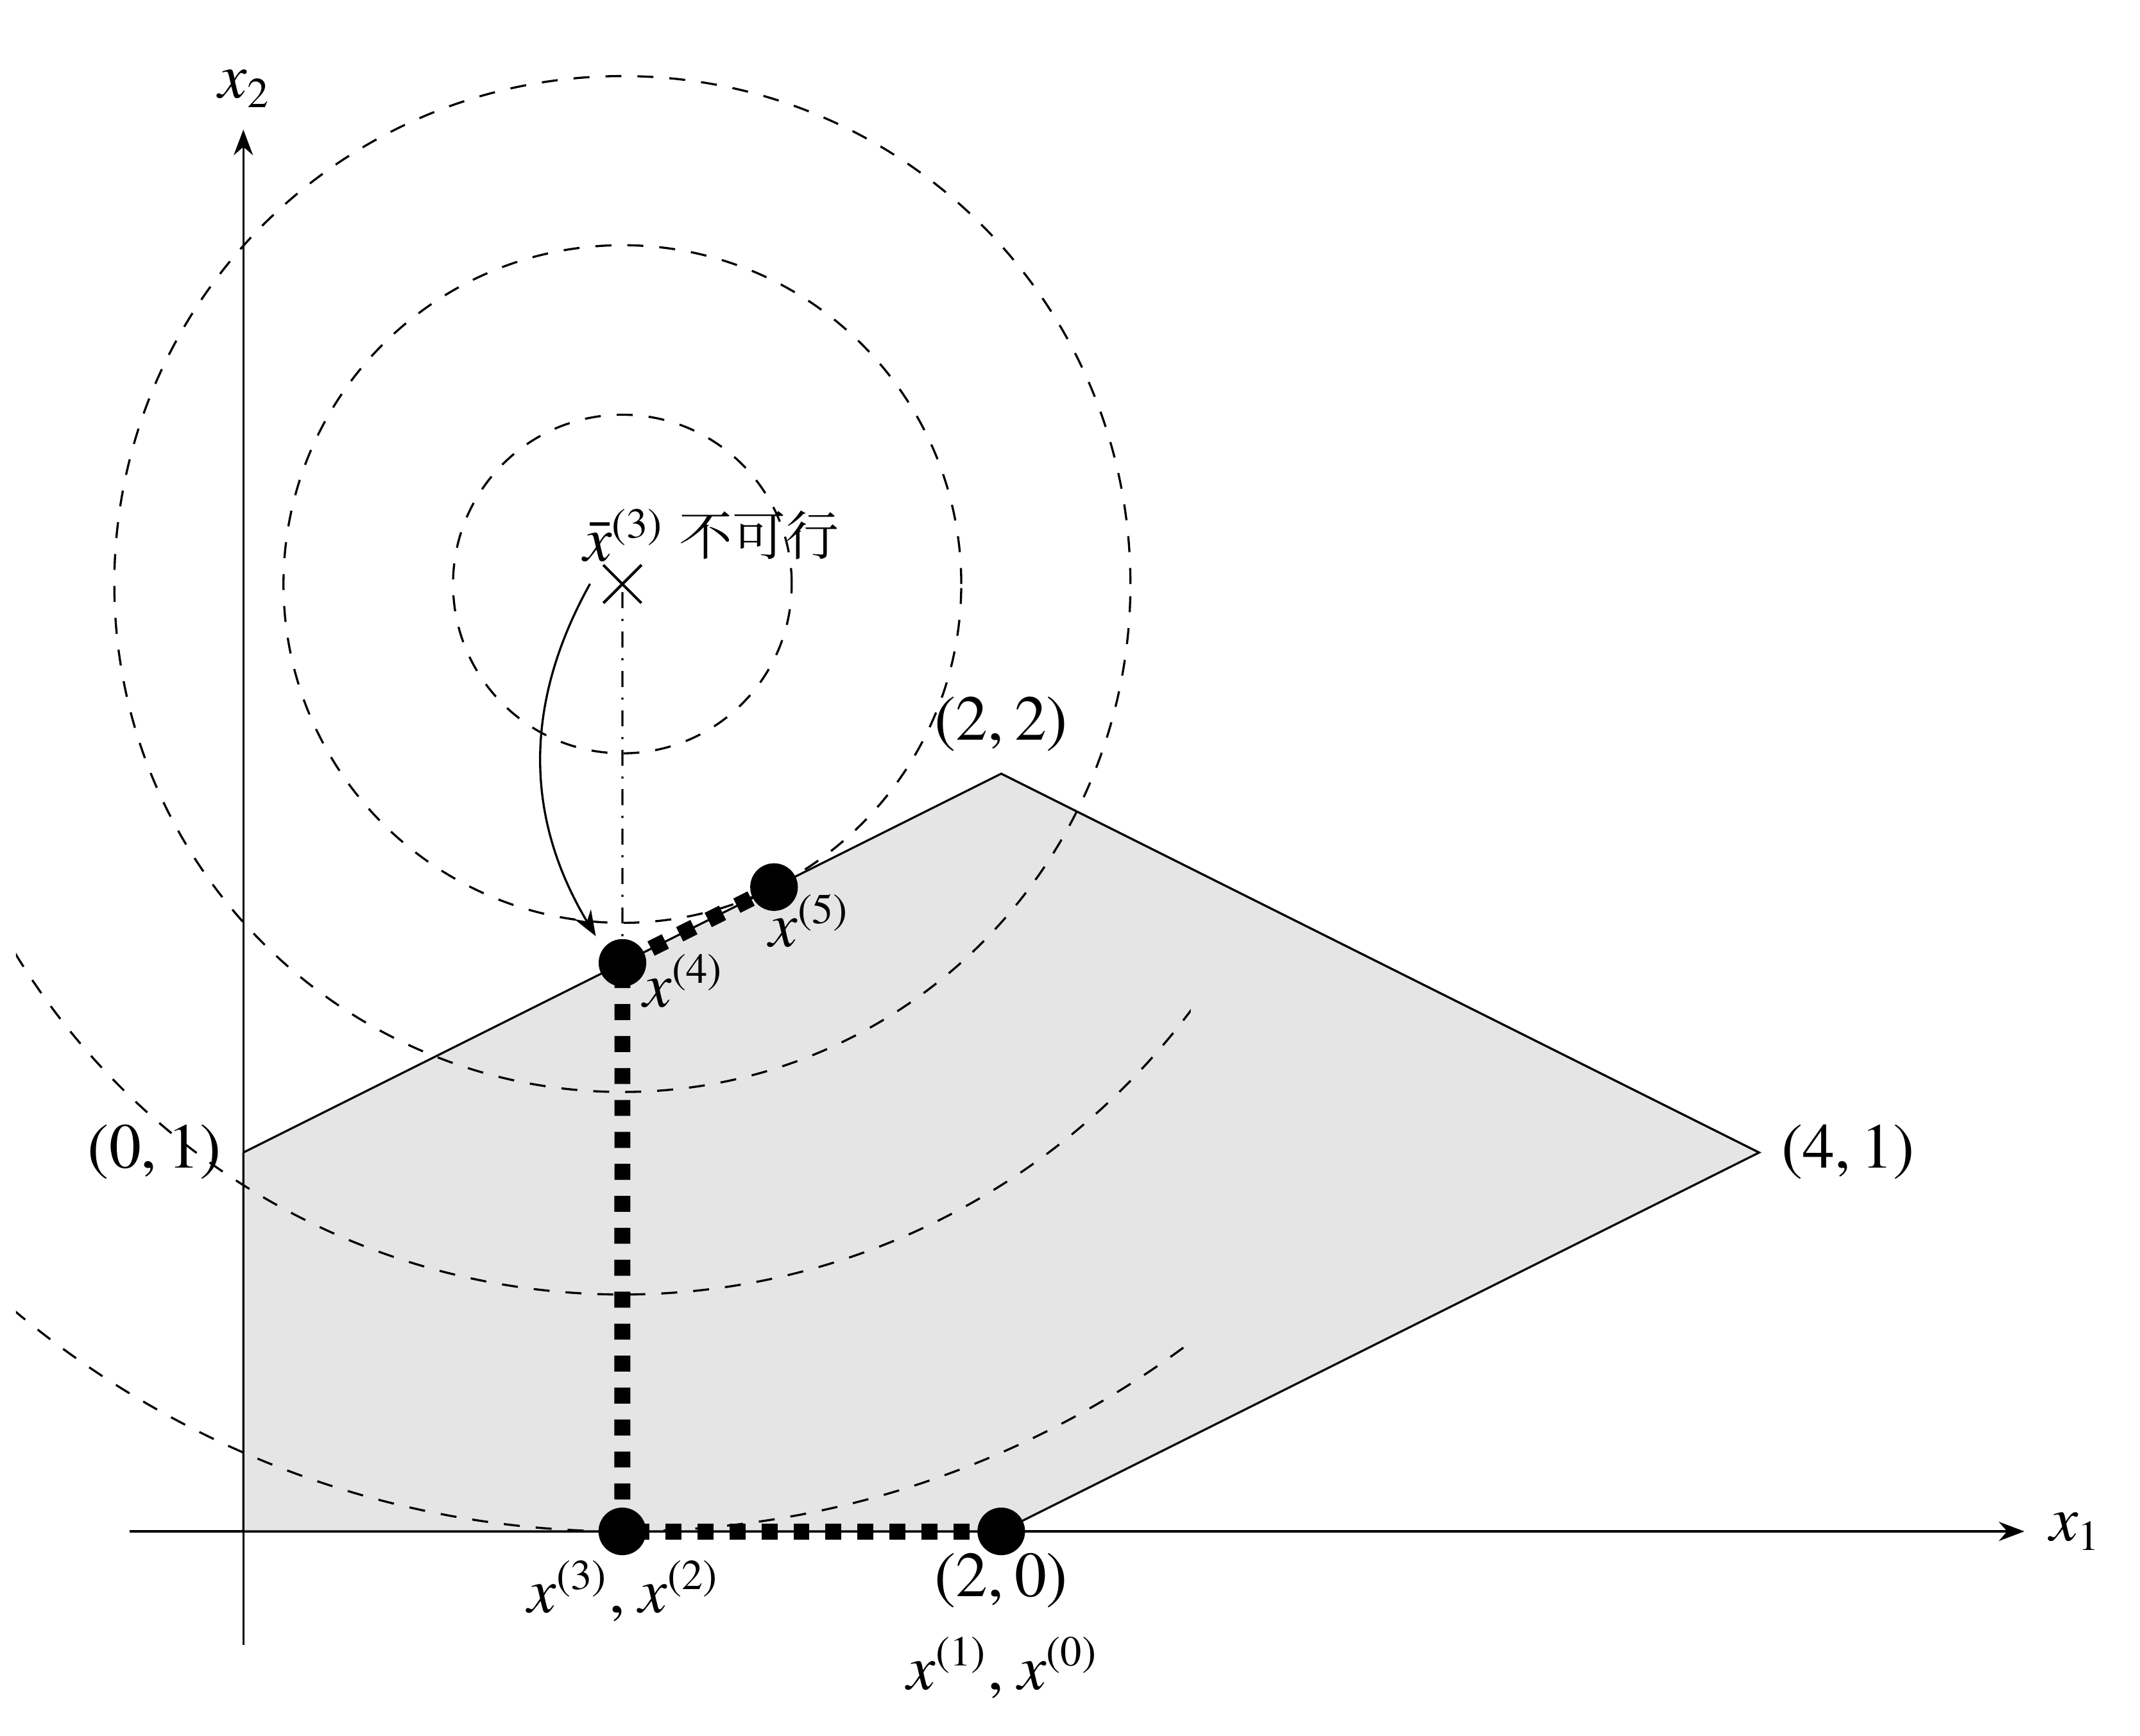
\includegraphics[width=0.75\textwidth]{fig-qp-active-set.png}
% \caption{积极集法求解例~\ref{eg:qp-active-set-algo} 的迭代示意图}
% \end{figure}

\newif\ifsteparrows
% \steparrowstrue
\steparrowsfalse

\begin{figure}[ht]
\centering
\larger[1]
\begin{tikzpicture}[scale=2.5, circle defined by/.style args={center #1 and point #2}{insert path={let \p1=($(#2)-(#1)$),\n1={veclen(\x1,\y1)} in (#1) circle[radius=\n1]}}]
% \draw[gray!30, thin, dashed] (-0.5, -0.5) grid (4.6, 3.9);
\coordinate (C) at (1, 2.5);
% coordinate axes
\draw[-{Stealth}] (-0.3, 0) -- (4.7, 0) node [right] {$x_1$};
\draw[-{Stealth}] (0, -0.3) -- (0, 3.7) node [above] {$x_2$};
% feasible region
\draw[fill=gray!20] (0, 1) node (p1) [left] {$(0, 1)$} -- (2, 2) node (p2) [above] {$(2, 2)$} -- (4, 1) node (p3) [right] {$(4, 1)$} -- (2, 0) node (p4) [below] {$(2, 0)$} -- (0, 0) -- (0, 1);
% iterations of the active-set algorithm
\node[below = -0.1 of p4] (x01) {${x}^{(1)}, {x}^{(0)}$};
\draw[dashed, line width=3] (2, 0) -- (1, 0) node (x23) [below] {${x}^{(3)}, {x}^{(2)}$};
\path[name path = line1] (0, 1) -- (2, 2);
\path[name path = vertical1] (1, 0) -- (1, 4);
\draw[dashed, line width=3, name intersections = {of = line1 and vertical1, by = {x4}}]  (1, 0) -- (x4);
\node[below right = -0.2 and -0.03 of x4] (xx4) {${x}^{(4)}$};
\draw[dashdotted, thin] (x4) -- (C) node[above] (barx3) {$\bar{{x}}^{(3)}$};
\draw plot[only marks,mark=x,mark size=2] (C);
\node[right = -0.2 of barx3] {\smaller 不可行};
\path (barx3) edge [draw, bend right, -{Stealth}] ([xshift=-2, yshift=2]x4);
\coordinate (c1) at (0, 1);
\coordinate (c2) at (2, 2);
\coordinate (x5) at ($(c1)!(C)!(c2)$);
\draw[dashed, line width=3] (x4) -- (x5);
\node[below right = -0.1 and -0.2 of x5] {${x}^{(5)}$};
\foreach \x in {(2,0), (1,0), (x4), (x5)} \draw[fill=black] \x circle (0.06);
% contour: circles
\begin{scope}
% \clip (-.6, -.3) rectangle (3, 3.2);
\draw[dashed, circle defined by=center C and point x5];
\coordinate (midx5) at ($(C)!0.5!(x5)$);
\draw[dashed, circle defined by=center C and point midx5];
\coordinate (p6) at ($(C)!1.5!(x5)$);
\draw[dashed, circle defined by=center C and point p6];
\end{scope}
% contour: arcs
\begin{scope}
\clip (-.6, -.3) rectangle (2.5, 1.9);
\coordinate (p7) at (1, 0);
\draw[dashed, circle defined by=center C and point p7];
\coordinate (p8) at ($(C)!0.75!(p7)$);
\draw[dashed, circle defined by=center C and point p8];
\end{scope}

% optional plots
\ifsteparrows
\path ([xshift=5]x01.south) edge [draw, bend left, -{Stealth}] ([xshift=-7]x01.south);
\path ([yshift=3]x01.west) edge [draw, -{Stealth}] ([xshift=-4, yshift=-3]x23.east);
\path ([xshift=5]x23.south) edge [draw, bend left, -{Stealth}] ([xshift=-7]x23.south);
\path (0.9, 0.1) edge [draw, bend left, -{Stealth}] (barx3.west);
\path ([xshift=-0.3, yshift=2]x4) edge [draw, bend left, -{Stealth}] ([xshift=-1, yshift=2]x5);
\fi
\end{tikzpicture}
\caption{积极集法求解例\ref{eg:qp-active-set-algo}~的迭代示意图}
\label{fig:active-set-eg}
\end{figure}


选取初始点~${x}^{(0)} = (2, 0)^T,$ 用~$1$ 至~$5$ 依次作为约束条件的指标. 在初始点~${x}^{(0)}$ 处, 约束~$3$ 和~$5$ 满足等式关系, 是积极约束, 所以初始积极集~$\mathcal{A} = \{ 3, 5 \}.$ 当前需要求解的等式问题~\eqref{eq:qp-active-set-1} 具体为
\begin{equation*}
\begin{array}{cl}
\min & q({x}) = (x_1 - 1)^2 + (x_2 - 2.5)^2, \\
{\rm s.t.} & x_1 - 2x_2 - 2 = 0, \\
& x_2 = 0,
\end{array}
\end{equation*}
或者来求解经过平移的问题~\eqref{eq:qp-active-set-2}, 具体形式如下
\begin{equation}
\label{eq:qp-active-set-eg-problem}
\begin{array}{cl}
\min & q({s}) = (s_1 + 1)^2 + (s_2 - 2.5)^2, \\
{\rm s.t.} & s_1 - 2s_2 = 0, \\
& s_2 = 0.
\end{array}
\end{equation}
很容易看到~${x}^{(0)}$ $($即~${s}^{(0)} = {0}$~$)$ 是该问题的解.
由式~\eqref{eq:qp-active-set-lambda} 求解积极约束的拉格朗日乘子, 即求解方程组
\begin{equation*}
\begin{bmatrix} 1 \\ -2 \end{bmatrix} \lambda_3^{(0)} + \begin{bmatrix} 0 \\ -1 \end{bmatrix} \lambda_5^{(0)} = \begin{bmatrix} -2 \\ 5 \end{bmatrix},
\end{equation*}
解得
\begin{equation*}
\lambda_3^{(0)} = -2, \lambda_5^{(0)} = -1, ~~\text{指标}~ q = \argmin\limits_{i \in \{ 3, 5 \}} \lambda_i^{(0)} = 3.
\end{equation*}
由于~$\lambda_q^{(0)} = \lambda_3^{(0)} = -2 < 0,$ 因此置
\begin{equation*}
{x}^{(1)} = {x}^{(0)} = (2, 0)^T,
\end{equation*}
同时将指标~$q = 3$ 从积极集中删去, 进入下一步迭代.

接下来需要求解等式问题
\begin{equation*}
\begin{array}{cl}
\min & q({s}) = (s_1 + 1)^2 + (s_2 - 2.5)^2, \\
{\rm s.t.} & s_2 = 0.
\end{array}
\end{equation*}
容易解得~${s}^{(1)} = (-1, 0)^T.$ 此时, 试探点~${x}^{(1)} + {s}^{(1)} = (1, 0)^T$ 是可行点, 于是可以置
\begin{equation*}
{x}^{(2)} = {x}^{(1)} + {s}^{(1)} = (1, 0)^T,
\end{equation*}
同时积极集~$\mathcal{A} = \{ 5 \}$ 保持不变, 进入下一步迭代.

容易验证~${x}^{(2)}$ 是接下来这一步要解的等式问题的可行解, 进而可计算得到相应的积极约束的拉格朗日乘子~$\lambda_5^{(2)} = -5.$ 此时, 约束~$5$ 变成非积极的, 积极集~$\mathcal{A}$ 变为空集~$\emptyset.$ 置
\begin{equation*}
{x}^{(3)} = {x}^{(2)} = (1, 0)^T
\end{equation*}
进入下一步迭代.

再次求解当前~$($经过平移$)$ 的等式约束问题~$($实际上已成为无约束问题$)$
\begin{equation*}
\min ~~ q({s}) = s_1^2 + (s_2 - 2.5)^2,
\end{equation*}
得解~${s}^{(3)} = (0, 2.5)^T.$ 试探点~${x}^{(3)} + {s}^{(3)} = (1, 2.5)^T$ 不是可行点,
因此需要以~${p}^{(3)} = {s}^{(3)}$ 为方向进行线搜索~${x}^{(3)} + \alpha_3 {p}^{(3)},$
并由式~\eqref{eq:qp-active-set-step-len-2} 以及式~\eqref{eq:qp-active-set-step-len-uniform} 算得最优步长~$\alpha_3 = 0.6,$ 以及相应阻滞约束的指标~$j = 1.$ 置
\begin{equation*}
{x}^{(4)} = {x}^{(3)} + \alpha_3 {p}^{(3)} = (1, 1.5)^T,
\end{equation*}
并将阻滞约束的指标~$j = 1$ 添加到积极集得~$\mathcal{A} = \{ 1 \},$ 进入下一步迭代.

继续求解当前的等式问题
\begin{equation*}
\begin{array}{cl}
\min & q({s}) = s_1 + (s_2 - 1)^2, \\
{\rm s.t.} & s_1 - 2s_2 = 0.
\end{array}
\end{equation*}
解得~${s}^{(4)} = (0.4, 0.2)^T.$ 相应的试探点~${x}^{(4)} + {s}^{(4)} = (1.4, 1.7)^T$ 可行, 于是得新的迭代点
\begin{equation*}
{x}^{(5)} = {x}^{(4)} + {s}^{(4)} = (1.4, 1.7)^T.
\end{equation*}
由于~${x}^{(5)}$ 是当前等式问题的可行点, 且解得积极约束的拉格朗日乘子~$\lambda_1^{(5)} = 0.8 > 0,$ 算法终止条件达成, 得原问题的最优解
\begin{equation*}
{x}^* = {x}^{(5)} = (1.4, 1.7)^T.
\end{equation*}
我们将以上每一步的数值结果总结在表~\ref{tab:active-set-eg} 中, 这样读者会对整个算法流程有更清晰的认知. 表中的``$\backslash$''表示当前迭代步不需要计算相应的量.
\begin{table}[H]
    \caption{积极集法求解例~\ref{eg:qp-active-set-algo} 数值结果}
    \label{tab:active-set-eg}
    \centering
    \begin{tabular}{cccccccccc}
    \hline
    $k$ & ${x}^{(k)}$ & $\mathcal{A}$ & ${s}^{(k)}$ & $\bar{{x}}^{(k)}$可行 & ${\lambda}^{(k)}$ & $q$ & $\alpha_k$ & $j$ & $q({x}^{(k)})$ \\
    \hline
    \multirow{2}{*}{$0$} & \multirow{2}{*}{$(2, 0)^T$} & \multirow{2}{*}{$\{ 3, 5 \}$} & \multirow{2}{*}{$(0, 0)^T$} & \multirow{2}{*}{$\checkmark$} & $\lambda_3^{(0)} = -2$ & \multirow{2}{*}{$3$} & \multirow{2}{*}{$0$} & \multirow{2}{*}{$\backslash$} & \multirow{2}{*}{$7.25$} \\
    & & & & & $\lambda_5^{(0)} = -1$ & & & \\
    $1$ & $(2, 0)^T$ & $\{ 5 \}$ & $(-1, 0)^T$ & $\checkmark$ & $\backslash$ & $\backslash$ & $1$ & $\backslash$ & $7.25$ \\
    $2$ & $(1, 0)^T$ & $\{ 5 \}$ & $(0, 0)^T$ & $\checkmark$ & $\lambda_5^{(2)} = -5$ & $5$ & $0$ & $\backslash$ & $6.25$ \\
    $3$ & $(1, 0)^T$ & $\emptyset$ & $(0, 2.5)^T$ & $\times$ & $\backslash$ & $\backslash$ & $0.6$ & $1$ & $6.25$ \\
    $4$ & $(1, 1.5)^T$ & $\{ 1 \}$ & $(0.4, 0.2)^T$ & $\checkmark$ & $\backslash$ & $\backslash$ & $1$ & $\backslash$ & $1$ \\
    $5$ & $(1.4, 1.7)^T$ & $\{ 1 \}$ & $(0, 0)^T$ & $\checkmark$ & $\lambda_1^{(5)} = 0.8$ & $\backslash$ & $\backslash$ & $\backslash$ & $0.8$ \\
    \hline
    \end{tabular}
\end{table}
\end{exam}


\subsection*{习题}
% finished

\begin{enumerate}

\item 写出二次规划问题
\begin{equation*}
\begin{array}{cl}
\text{maximize} & q(\V{x}) = 6x_1 + 4x_2 - 13 - x_1^2 - x_2^2, \\
\text{subject to} & x_1 + x_2 \leqslant 3, \\
& x_1, ~ x_2 \geqslant 0
\end{array}
\end{equation*}
的KKT条件. 写出上述规划问题的对偶问题, 以及对偶问题的对偶问题.

\item 分别利用直接消元法以及正交分解法(广义消元法)求解如下的等式约束的二次规划问题, 并检查它们得到的解是否相同.
\begin{equation*}
\begin{array}{cl}
\text{minimize} & q(x) = x_1^2 + x_2^2 + x_3^2 + 2x_3, \\
\text{subject to} & x_1 + 2x_2 - x_3 = 4, \\
& x_1 - x_2 + x_3 = -2.
\end{array}
\end{equation*}

\item 设$\V{x}^*$是二次规划问题~\eqref{eq:quadratic-programming-1}~的解, 证明$\V{x}^*$也是下列线性规划问题的解
\begin{equation*}
\begin{array}{cl}
\text{minimize} & \V{x}^T \left( G \V{x}^* + \V{d} \right), \\
\text{subject to} & \V{a}_i^T \V{x} = b_i, ~~ i \in \mathcal{E}, \\
& \V{a}_i^T \V{x} \leqslant b_i, ~~ i \in \mathcal{I},
\end{array}
\end{equation*}

\item 令$A$是一个$n \times m$的列满秩的矩阵, 求$n$维空间中一点$\V{x}_0$到$\{ x : ~ A^T \V{x} = \V{b} \}$最短距离的问题可以表述为如下的等式约束二次规划问题
\begin{equation*}
\begin{array}{cl}
\text{minimize} & \frac{1}{2} \left( \V{x} - \V{x}_0 \right)^T \left( \V{x} - \V{x}_0 \right), \\
\text{subject to} & A^T x = b,
\end{array}
\end{equation*}
证明该问题的解以及拉格朗日乘子为
\begin{equation*}
\begin{aligned}
\V{x}^* & = \V{x}_0 + A \left( A^T A \right)^{-1} \left( \V{b} - A^T \V{x}_0 \right), \\
\V{\lambda}^* & = \left( A^T A \right)^{-1} \left( \V{b} - A^T \V{x}_0 \right),
\end{aligned}
\end{equation*}
并进一步证明当$A = \V{a}$是一个列向量时, 从点$\V{x}_0$到$\R^n$中的超平面$\{ x : ~ \V{a}^T \V{x} = b \}$最短距离等于$\dfrac{\lvert b - \V{a}^T \V{x} \rvert}{\lVert \V{a} \rVert_2}.$

\item 设$G$是$n$阶可逆方阵, $A$是$n\times m$的矩阵且$A$列满秩. 令$K = \begin{bmatrix} G & A \\ A^T & 0 \end{bmatrix}.$ 证明
\begin{itemize}
    \item[(1)] 方阵$K$可逆;
    \item[(2)] 方阵$K$的逆矩阵可以由式~\eqref{eq:quadratic-programming-kkt-inv-1}~给出.
\end{itemize}

\item 考虑等式约束的二次规划问题~\eqref{eq:quadratic-programming-eq-constrained}. 设$G$半正定, $A \neq 0$列满秩, $Z$为矩阵$A$的列零空间的一组基构成的矩阵, $K = \begin{bmatrix} G & A \\ A^T & 0 \end{bmatrix}$是KKT矩阵. 证明
\begin{itemize}
    \item[(1)] KKT矩阵$K$总是不定的;
    \item[(2)] 若进一步假设既约Hessian阵$Z^T G Z$正定, 则KKT矩阵$K$非奇异, 并且其逆可由式~\eqref{eq:quadratic-programming-kkt-inv-2}~给出;
    \item[(3)] 若既约Hessian阵$Z^T G Z$正定, 该二次规划问题有唯一极小点, 该点就是唯一的全局最优解;
    \item[(4)] 假设方程$A^⊤ \V{x} = \V{b}, ~ G \V{x} + A \V{\lambda} = − \V{d}$有解. 如果既约Hessian阵$Z^T G Z$半正定且奇异, 那么问题~\eqref{eq:quadratic-programming-eq-constrained}~有无穷多解;
    \item[(5)] 如果既约Hessian阵$Z^T G Z$不定, 或者方程$G \V{x} + A \V{\lambda} = − \V{d}$无解, 则问题~\eqref{eq:quadratic-programming-eq-constrained}~的目标函数无界.
\end{itemize}

\item 证明二次规划问题~\eqref{eq:quadratic-programming-1}~的KKT条件~\eqref{eq:quadratic-programming-kkt}~与利用积极集表达的KKT条件~\eqref{eq:qp-active-set-kkt}~等价.

\item 分别以$\{3\},$ $\{5\},$ 以及$\emptyset$为初始积极集$\mathcal{A},$ 用积极集法求解例\ref{eg:qp-active-set-algo}~中的不等式约束的二次规划问题.

\item 假设积极集法选取的初始积极集$\mathcal{A}$中约束的梯度是线性无关的, 即$\{ \V{a}_i: ~ i \in \mathcal{A} \}$是线性无关组, 并且在随后某一步, 根据式~\eqref{eq:qp-active-set-step-len-2}~添加了一条阻滞约束$j$到积极集$\mathcal{A}$中. 证明阻滞约束的梯度$\V{a}_j$与该集合中其余向量线性无关.

另一方面, 当我们从积极集中按式~\eqref{eq:qp-active-set-inactive-index}~删去一条非积极约束, 显然不会改变当前积极集中梯度向量组成线性无关组这一性质. 由此, 由归纳法可知, 积极集法的迭代步中关于积极集的修正策略, 可以移植保持积极集对应的约束的梯度向量组线性无关这一性质.

\item 假设在积极集法的第$k$步, 我们按式~\eqref{eq:qp-active-set-inactive-index}~删去一条非积极约束$q.$ 证明下一步的搜索方向$\V{p}^{(k+1)}$是目标函数$q(\V{x})$的严格下降方向(即$\left( \V{p}^{(k+1)} \right)^T \V{g}^{(k+1)} < 0$), 且该方向是严格可行的(即$\left( \V{p}^{(k+1)} \right)^T \V{a}_q > 0$).

\item 利用矩阵增加或者减少一行时的QR分解的更新方法编写积极集法\ref{algo:active-set}~的程序, 并用其求解二次规划问题
\begin{equation*}
\begin{array}{cl}
\text{minimize} & x_1^2 + 2x_2^2 -2x_1x_2 - 2x_1 - 6x_2, \\
\text{subject to} & -x_1 - x_2 \leqslant -2, \\
& -x_1 + 2x_2 \leqslant 2, \\
& -x_1 \leqslant 0,\\
& -x_2 \leqslant 0.
\end{array}
\end{equation*}
选取三个初始点: 一个在可行域的内部(例如$(3, 1)^T$); 一个在顶点(例如$(\frac{2}{3}, \frac{4}{3})^T$); 一个在可行域的边界上, 但不是顶点(例如$(4, 0)^T$).

提示: 可以利用Matlab的\texttt{qr.m}, \texttt{qrinsert.m}和\texttt{qrdelete.m}函数, 或者利用Python \texttt{scipy}软件包的\texttt{scipy.linalg.qr}, \texttt{scipy.linalg.qr\_insert}和\texttt{scipy.linalg.qr\_delete}函数.

% \item 用积极集法求解下面的二次规划问题

\end{enumerate}


% \bibliographystyle{sbc}
% \bibliography{references}
\printbibliography[heading=bibintoc, title=参考文献]

\end{document}
